% Created 2021-01-24 Sun 22:49
% Intended LaTeX compiler: pdflatex
\documentclass[11pt]{article}
\usepackage[utf8]{inputenc}
\usepackage[T1]{fontenc}
\usepackage{graphicx}
\usepackage{grffile}
\usepackage{longtable}
\usepackage{wrapfig}
\usepackage{rotating}
\usepackage[normalem]{ulem}
\usepackage{amsmath}
\usepackage{textcomp}
\usepackage{amssymb}
\usepackage{capt-of}
\usepackage{hyperref}
\usepackage{minted}
\hypersetup{colorlinks=true, linkcolor=black, filecolor=red, urlcolor=blue}
\usepackage[turkish]{babel}
\author{Eren Hatırnaz}
\date{15 Mart 2020}
\title{Yazılım Gündemi - 2020/10\\\medskip
\large 9-15 Mart 2020}
\hypersetup{
 pdfauthor={Eren Hatırnaz},
 pdftitle={Yazılım Gündemi - 2020/10},
 pdfkeywords={},
 pdfsubject={},
 pdfcreator={Emacs 27.1 (Org mode 9.3)},
 pdflang={Turkish}}
\begin{document}

\maketitle
\tableofcontents \clearpage\shorthandoff{=}

\begin{center}
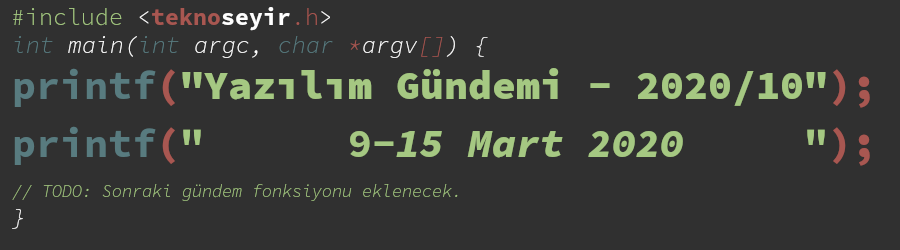
\includegraphics[width=.9\linewidth]{gorseller/yazilim-gundemi-banner.png}
\end{center}

\begin{center}
\href{../09/yazilim-gundemi-2020-09.pdf}{< Önceki Gündem} | \textbf{9-15 Mart 2020} | \href{../11/yazilim-gundemi-2020-11.pdf}{Sonraki Gündem >}

\href{https://teknoseyir.com/blog/yazilim-gundemi-2020-10}{TeknoSeyir'de Oku}
\end{center}

\section{Microsoft, Visual Basic'i artık \href{https://devblogs.microsoft.com/vbteam/visual-basic-support-planned-for-net-5-0/}{geliştirmeyeceğini duyurdu}}
\label{sec:orgd0f8a34}
\begin{center}
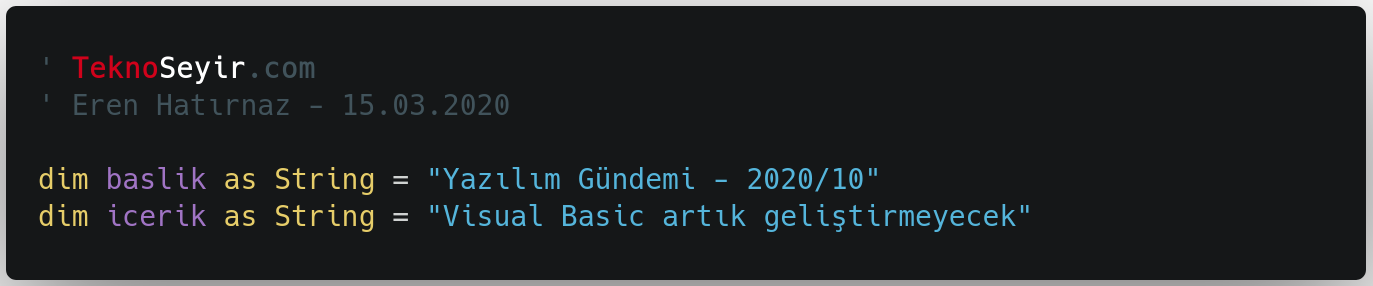
\includegraphics[width=.9\linewidth]{gorseller/visual-basic-gelistirme.png}
\end{center}

Microsoft'un açık kaynak camiasına açılmasıyla birlikte gelen köklü
değişikliklerden biri olan .NET Core projesinin artık Microsoft'un ana
uygulama geliştirme çatısı haline geldiğini biliyoruz. Geçtiğimiz yazılım
gündemi yazılarında da (bkz: \href{../../2019/14/yazilim-gundemi-14.pdf}{Yazılım Gündemi - 14}) .NET Framework API'lerinin
.NET Core'a aktarılmasının tamamlandığını haber vermiştim. Yine başka bir
yazıda ise .NET Core çatısının artık .NET 5 ismiyle hayatına devam edeceğini
duyurmuştum. Bu hafta ise Microsoft .NET Takımı, Visual Basic için .NET 5
planlarını açıkladılar. .NET 5 içerisinde de Visual Basic desteği şu uygulama
tipleri için olacak:

\begin{itemize}
\item Class Library
\item Console
\item Windows Forms
\item WPF
\item Worker Service
\item ASP.NET Core Web API
\end{itemize}

Bunların dışında kalan WebForms, Workflow ya da WCF gibi uygulama tipleri ise
.NET 5 sürümünde yer almayacak. Eğer bu tiplerde geliştirdiğiniz uygulamalar
varsa Microsoft, .NET 5 çatısına geçirmenizi tavsiye ediyor. Eğer kurumsal
müşteri iseniz de bu konuda destek veriyor.

Aynı blog yazısında duyurulan bir diğer gelişme ise, artık Visual Basic'in dil
olarak geliştirilmeye devam edilmeyeceği haberi oldu. İlerleyen .NET
sürümlerinde gelecek olan özellikler artık Visual Basic'e eklenmeyecek.
Microsoft zaten 2017'de C\# ve VB.NET'in eşit geliştirilmesini bıraktığını,
C\#'a ağırlık \href{https://www.thurrott.com/dev/89874/microsoft-outlines-development-language-strategy}{vereceğini duyurmuştu}. Dolayısıyla pek de sürpriz bir gelişme
değil yani. Ben de programlamaya ilgi duyduğum orta okul yıllarında biraz
haşır neşir olduğum bir dildi fakat sonrasında C\#'a geçmiştim ben de.

Eğer hala Visual Basic ile geliştirmeye devam ettiğiniz uygulamalar varsa
sistemin durumuna göre bir tekrar gözden geçirip, yeni kararlar vermekte fayda
var fakat yine de unutmayalım ki: "Çalışıyorsa dokunma" :)
\section{Twitter, Geliştirici Yönergelerini akademik araştırmaları daha iyi \href{https://techcrunch.com/2020/03/10/twitter-rewrites-developer-policy-to-better-support-academic-research-and-use-of-good-bots/}{desteklemek için güncelledi}}
\label{sec:org2b5d74c}
Twitter, bu hafta içerisinde kendi platformu üzerinde uygulama geliştiren
geliştiricilerin uyması gereken kuralları güncelledi. Yani Developer Policy
güncellendi ve sadeleştirildi. Önceden 8 bölümden oluşan metin artık 4 bölüme
inmiş durumda. Bu değişiklikle birlikte öne çıkan iki önemli konu mevcut.
Birisi Twitter artık akademik araştırmalar için verilerin kullanılması ve
yeniden dağıtılması konusunda daha anlayışlı, diğeri ise Twitter'ın artık
"iyi" botlara sıcak bakmaya başlaması.

Twitter'daki herkese açık paylaşımlar artık ticari olmayan akademik
araştırmalar için kullanılabilecek. Üstelik yenilenen policy sayesinde artık
araştırmada sonuç üretmek için kullandığımız tweet'lerin ya da kullanıcıların
id'lerini de çalışmamızla birlikte yeniden dağıtabiliyoruz. Böylece akran
değerlendirmesi sırasında aynı tweet ve kullanıcılar kullanılarak, sizin elde
ettiğiniz sonucu başkaları da elde edebilecekler.

Veri erişilebilirliğiyle ilgili bu değişikliklerin yanı sıra artık Twitter'da
bot hesapları da yasal olarak oluşturabileceğiz. "Bot" hesaplardan kast
ettiğim tabii ki de otomatik beğeni ya da RT yapan botlar değil. Twitter şu
iki botu örnek olarak göstermiş mesela: \href{https://twitter.com/earthquakesSF}{EarthQuakesSF} ve \href{https://twitter.com/everycolorbot}{EveryColorBot}.
İnsanlara faydalı amaçlar için geliştirilmiş botlar olması gerekiyor. Bunu tam
olarak nasıl belirleyeceklerini bilmiyorum, policy metnini okuyacak vaktim
olmadı ama üstesinden geleceklerdir sanırım.

Ayrıca Twitter, uygulamalar ile ilgili bazı istatistikler de paylaştı.
Twitter, Temmuz 2018'den beri bir milyondan fazla uygulamayı review etmiş ve
\%75'ini kabul etmiş. Ek olarak son 6 ayda 144.000 uygulama da kötü amaçlı
kullanıldıkları için kaldırılmış.
\section{Bootstrap 5 ile gelecek bazı özellikler \href{https://themesberg.com/blog/design/bootstrap-5-release-date-and-whats-new}{belli oldu}}
\label{sec:orgb66c676}
Ben dahil birçok back-end geliştiricisinin onlarca projede imdadına yetişen
arayüz sistemi Bootstrap \href{https://github.com/twbs/bootstrap/projects/11}{son hızıyla geliştirilmeye devam ediyor}. Henüz resmi
bir açıklama olmasa da Bootstrap 5 sürümünün bahar aylarının sonlarına doğru
yayınlanması bekleniyor. Bu sırada ise GitHub üzerindeki değişiklikleri
incelediğimizde gördüğümüz bazı şeyler var. Bunlar şu şekilde:

\begin{itemize}
\item jQuery bağımlılığı kaldırıldı
\item Internet Explorer 10 ve 11 desteği kaldırıldı
\item SVG icon kütüphanesi eklendi
\end{itemize}

Bu üçünün dışında daha birçok değişikliğin de uygulandığını \href{https://github.com/twbs/bootstrap/projects/11}{bu proje
sayfası}ndan görebilirsiniz. Internet Explorer 10 ve 11 desteğinin
kaldırılmasına şaşırmadık elbette. Aslında bakarsanız jQuery desteğinin
kalmasına da şaşırmadım ben. Son 3-4 yıldır VueJS ve React gibi kütüphanelerin
yaygınlaşmasıyla birlikte zaten jQuery'yi çok nadir görüyorduk. Bootstrap
ekibi de artık bunun farkına varmış olacak ki artık kullanmamaya karar
vermişler.

Diğer değişiklikler ve özellikler için konu başlığına eklediğim bağlantıya ya
da \href{https://github.com/twbs/bootstrap/projects/11}{proje sayfası}na göz atabilirsiniz.
\section{Django yönetim \href{https://www.djangoproject.com/weblog/2020/mar/12/governance/}{şeklini değiştirdi}}
\label{sec:org8e8f7ff}
Belirli bir büyüklüğe ulaşan her programlama dili ve framework gibi Django'nun
da artık bazı kararlar vermesi gerekiyordu ve bu hafta içerisinde
yayınladıkları blog yazısıyla birlikte yönetim sistemiyle ilgili "DEP"
belgesinin \href{https://github.com/django/deps/blob/master/accepted/0010-new-governance.rst}{kabul edilmiş halini yayınladılar}.

Açıkcası Django ile hiç proje geliştirmediğim için yapısına da hakim değilim
fakat okuduklarımdan anladığım kadarıyla önceden bir "ana geliştirici akımı"
varmış ve genelde geliştirmeler bu kişiler tarafından yapılıyor ya da
dışarıdan gelen katkıları yine bu kişiler değerlendiriyormuş. Fakat artık
projenin de fazlaca büyümesiyle birlikte bu süreç zorlaşmış olacak ki farklı
roller getirerek görevleri ve sorumlulukları dağıtmayı tercih etmişler. Ayrıca
"Techninal Board" gibi komitelerin de kurulacağını belirtmişler. Anlayacağız
artık Django geliştirme süreci daha sistematik bir şekilde işleyecek.

Yeni yönetim şekliyle ilgili detaylara konu başlığına eklediğim bağlantı
üzerinden ulaşabilirsiniz.
\section{Unicode 13.0.0 \href{https://unicode.org/versions/Unicode13.0.0/}{sürümü yayınlandı}}
\label{sec:orgfa47e49}
Aynı zamanda uygulamalar üzerinde kullandığımız "emoji"lerin de standardı olan
Unicode standardının 13.0 sürümü yayınlandı. Bazı değişiklikler şu şekilde:

\begin{itemize}
\item 5.930 yeni karakter eklemesiyle birlikte artık Unicode toplam 143.856
karakter barındırıyor,
\item 55 yeni "emoji" eklenmiş. Yeni emojilere \href{https://unicode.org/emoji/charts-13.0/emoji-released.html}{bu adresten} göz atabilirsiniz.
\end{itemize}
\section{Next.js kütüphanesinin 9.3 \href{https://nextjs.org/blog/next-9-3}{sürümü yayınlandı}}
\label{sec:org7c47022}
\begin{itemize}
\item Yeni nesil statik site oluşturma desteği,
\item Ön-izleme modu,
\item Global stillendirme için gömülü SASS desteği (\texttt{.scss}),
\item Komponent bazında stillendirme için SASS Modül desteği (\texttt{.module.scss}),
\item 404 sayfaları için otomatik statik optimizasyon,
\item Tüm runtime sadece 32 kB,
\item Toplulukla ilgili tartışmalar artık \href{https://github.com/zeit/next.js/discussions}{GitHub Discussions üzerinde} olacak.
\end{itemize}

Özelliklerin detayları için konu başlığına eklediğim bağlantıya
tıklayabilirsiniz.
\newpage
\section{Visual Studio Code Şubat 2020 (v1.43) \href{https://code.visualstudio.com/updates/v1\_43}{sürümü yayınlandı}}
\label{sec:org91b5c68}
\begin{figure}[htbp]
\centering
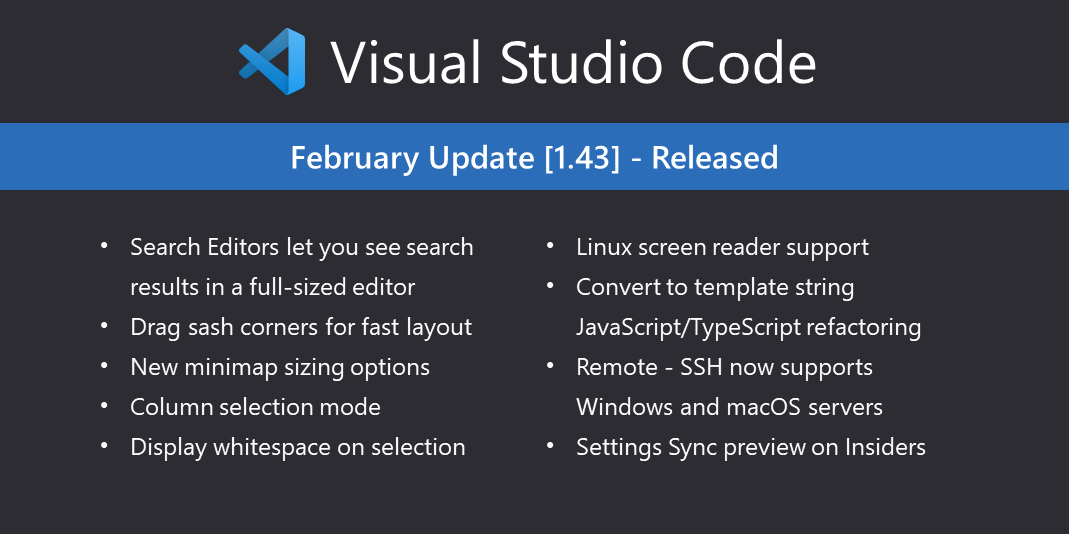
\includegraphics[width=.9\linewidth]{gorseller/vscode-1-43.png}
\caption{Visual Studio Code editörünün Şubat 2020 sürümüyle birlikte gelen özellikler}
\end{figure}
\section{Diğer Haberler}
\label{sec:orgb3b15ab}
\begin{itemize}
\item Korona virüsü nedeniyle ertelenen konferanslar ve etkinlikler:
\begin{itemize}
\item PHPKonf İstanbul yaz aylarına \href{https://2020.phpkonf.org/updates.html}{ertelendi}. Yeni tarihler ilerleyen
haftalarda duyurulacak.
\item Apple, WWDC20 etkinliğini \href{https://developer.apple.com/news/?id=03132020a}{yaz aylarına erteledi}.
\item Angular Turkey etkinliğini \href{https://twitter.com/ngTurkiye/status/1237659540889522176}{ileri bir tarihe erteledi}.
\end{itemize}
\item Atlassian, Syndney ofisini kapattı ve bir sonraki duyuruya kadar evden
çalışma düzenine \href{https://mobile.twitter.com/Atlassian/status/1237996563953324032}{geçtiklerini duyurdu}.
\item Microsoft SMBv3'de kritik bir \href{https://kb.cert.org/vuls/id/872016/}{güvenlik açığı keşfedildi}.
\item Bill Gates, Microsoft'un \href{https://www.prnewswire.com/news-releases/microsoft-announces-change-to-its-board-of-directors-301023293.html}{yönetim kurulundan ayrıldı}.
\item GitHub CEO'su, sunucularının bir kısmını \href{https://foldingathome.org/2020/02/27/foldinghome-takes-up-the-fight-against-covid-19-2019-ncov/}{Folding@Home projesi} için
\href{https://mobile.twitter.com/natfriedman/status/1237466267998543872}{ayırdığını duyurdu}.
\item Netflix, kendi geliştirdiği AV1 encoder ve decoder'i \href{https://netflixtechblog.com/svt-av1-an-open-source-av1-encoder-and-decoder-ad295d9b5ca2}{açık kaynak olarak
yayınladı}. \href{https://github.com/OpenVisualCloud/SVT-AV1/}{GitHub Deposu}
\item Amazon, AWS HTTP APIs hizmetini \href{https://aws.amazon.com/tr/blogs/compute/building-better-apis-http-apis-now-generally-available/}{beta'dan çıkardı}.
\item InfoQ sitesi, \href{https://www.infoq.com/articles/javascript-web-development-trends-2020/}{JavaScript ve Web Geliştirme Trendleri 2020} raporunu
yayınladı.
\item Microsoft, .NET Core Uninstall Tool aracını \href{https://devblogs.microsoft.com/dotnet/announcing-the-net-core-uninstall-tool-1-0/}{tanıttı}.
\item Silverlight açık kaynak olarak geri döndü: \href{https://www.opensilver.net/announcements/introducing-opensilver.aspx}{OpenSilver}.
\item Google: "\href{https://opensource.googleblog.com/2020/03/webassembly-brings-extensibility-to.html?m=1}{WebAssembly, internet proxy'lerine genişletilebilirlik
kazandırıyor}".
\item Rust programlama dilinin 1.42.0 \href{https://blog.rust-lang.org/2020/03/12/Rust-1.42.html}{sürümü duyuruldu}.
\item GCC 9.3 \href{https://lists.gnu.org/archive/html/info-gnu/2020-03/msg00006.html}{sürümü yayınlandı}.
\item react-query v1.0.27 \href{https://github.com/tannerlinsley/react-query/blob/master/CHANGELOG.md\#1027}{sürümü çıktı}.
\item Memcached 1.6.0 \href{https://github.com/memcached/memcached/wiki/ReleaseNotes160}{sürümü çıktı}.
\item Ionic CLI 6.2.1 \href{https://github.com/ionic-team/ionic-cli/releases/tag/\%2540ionic\%252Fcli\%25406.2.1}{sürümü çıktı}.
\end{itemize}
\section{Lisans}
\label{sec:org75984f8}
\begin{center}
\begin{center}

\includegraphics[height=1.5cm]{../../../img/CC_BY-NC-SA_4.0.png}
\end{center}

\href{yazilim-gundemi-2020-10.pdf}{Yazılım Gündemi - 2020/10} yazısı \href{https://erenhatirnaz.github.io}{Eren Hatırnaz} tarafından \href{http://creativecommons.org/licenses/by-nc-sa/4.0/}{Creative Commons
Atıf-GayriTicari-AynıLisanslaPaylaş 4.0 Uluslararası Lisansı} (CC BY-NC-SA 4.0)
ile lisanslanmıştır.
\end{center}
\end{document}
